\documentclass[a4paper,10pt]{article}
\usepackage[francais]{babel}
\usepackage[utf8]{inputenc}
\usepackage[T1]{fontenc}
\usepackage{graphicx}
\usepackage{amsmath}
\usepackage{amssymb}
\usepackage{hyperref}
\usepackage{graphics}
\usepackage{listings}

%opening
\title{Problème combiné de localisation, routage et gestion des stocks}
\author{Seydou coulibaly}
\date{Mai 2016}
\begin{document}
\maketitle
\newpage
\begin{abstract}

Resumé

\paragraph{} 
Mot-cl\'es : problème d'inventaire, probléme de localisation, problème de routage, heuristique, methodes exactes, CPLEX.
\end{abstract}
\newpage
\section{Introduction}

Très longuement dans la litterature, des problèmes de Localisations, de Routages, ou d'Inventaires ont fut l'objet des thematiques de recherches 
dans plusieurs laboratoires et entreprise à travers le monde. Divers résultats ont été obtenus pour ces problèmes d'optimisation combinatoire
notament l'idée de l'association de plusieurs de ces problèmes (Localisation-Routage, Routage-Inventaire, Localisation-Inventaire) afin d'élaborer toujours de meilleurs décisions
strategiques, tactiques et operationnelles pour les entreprises. De la même idée (faire de meilleurs décisions), quelques experts ont eu l'idée de se 
pencher sur la combinaison des  trois problèmes ci-dessus formant ainsi le LIRP (Location, Invetory and Routing Problem), un problème très 
present dans le domaine de la logistique pour les entreprises industrielles.
\subsection*{Hypothèse I}
Dans tout ce qui va suivre, on suppose qu'on dispose d'une usine, d'un ensemble de depôts dispersés dans une region donnée et de plusieurs clients.
Les produits sont fabriqués puis acheminer de l'usine aux depôts où ils peuvent être stocker. L'usine peut ne pas être proche des depôts et ces derniers
assurent la livraison des produits au clients en fonction de leur demande et de leur état de stocks.
\subsection*{Problème de Localisation}
Dans ce problème, on s'interesse à la localisation des depôts à ouvrir parmi un nombre fini de depots, chacun ayant un côut d'installation et 
un espace (superficie) dans lequel il peut livrer ou fournir des clients. L'objectif est de minimiser le coût total d'installation des sites à ouvrir 
tout en s'assurant de satisfaire tous les clients sans exception. Il existe plusieurs variantes de ce problème dans la litterature parmi lesquelles
des contraintes de capacités sur les depôts à ouvrir.
\subsection*{Problème de Routage}
Le problème de routage est le problème dans lequel on cherche à trouver la route ayant la distance la plus minimale afin de l'emprunter. Chaque route 
passe par un ensemble de points qui peuvent être des depôts ou des clients. Plusieurs variantes en existe comme le TSP (où un visiteur fait le tour d'un
ensenble de ville en passant qu'une et une seule fois par une ville donnée), le VRP (Vehicule Routing Problem), CVRP (Capacited Vehicule Routing Problem)
,  etc. Chaque variante ajoute sa touche de contraintes.
\subsection*{Problème d'Inventaire}
Quant au problème d'inventaire, il cherche à decider de la quantité de commande à éffectuer à un temps t pour satisfaire la demande des clients. 
Cette quantité est contraint par une capacité de stocks du site dans lequel il sera posé . Un coût est associé à chaque quantité de stockage ainsi 
qu'à chaque commande éffectuée, l'objectif est de trouver cette quantité de commande au temps t minimisant le coût total sur un horizon fini. Plusieurs variantes en existe également.
\begin{figure}[h]
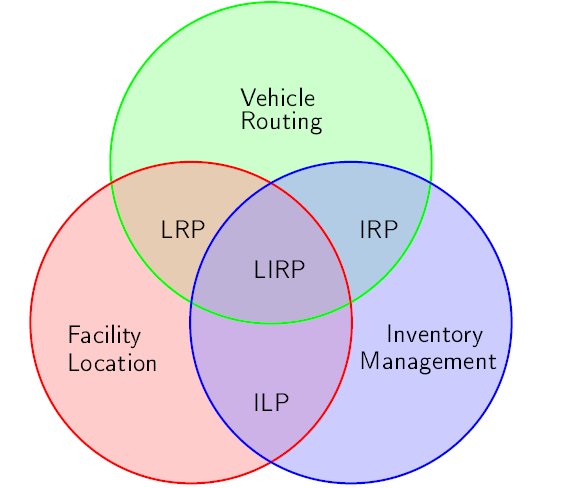
\includegraphics{lirp.PNG}
\caption{\label{lirp} \textbf{Location + Inventory + Routing = LIRP \cite{}}}
\end{figure}
\section{Modèle LIRP}
\paragraph{}
Le premier modèle mathématiques connu du problème LIRP a été réalisé par \emph{ Liu and Lee} (2003) \cite{} puis en 2005 
\emph{Liu and Lin} \cite{} ont proposé une metaheuristique hybribe (recherche tabou et recuit simulé ) pour le resoudre. Des années évoluant,
d'autres chercheurs s'y sont intéressé et ont presenté des solutions nouvelles comme \emph{Ambrosino Scutella} (2005) \cite{}, 
\emph{Ahmadi-Javid and Seddighi} (2012) \cite{} , \emph{Guerrero et al} (2013) \cite{} .

\subsection{Topologie du modèle}
Plusieurs variantes existant pour chacun des sous-problèmes formant le LIRP, un choix s'impose sur les types de contraintes à adopter
et le modèle à elaborer. Le schema \ref{topology} ci-dessous illustre quelques variantes possible du modèle.
\begin{figure}[h]
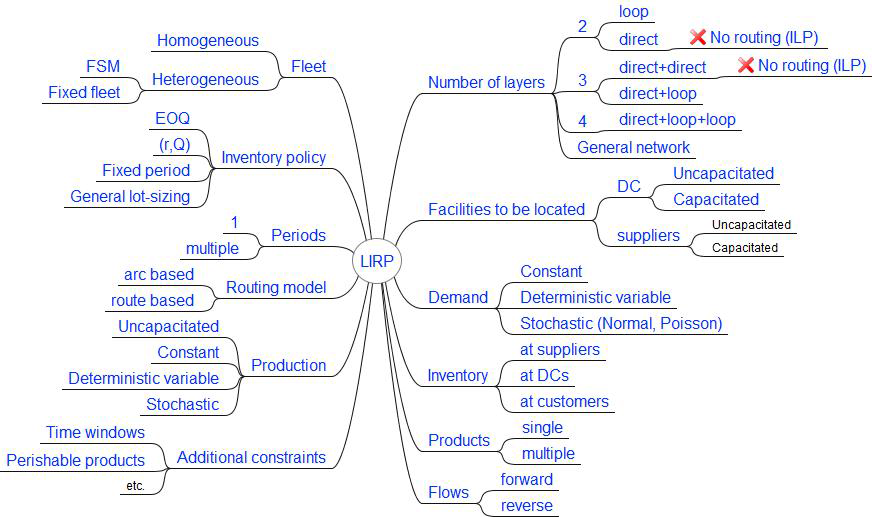
\includegraphics[width=16cm]{topology.png}
\caption{\label{topology} \textbf{Topologie du modèle LIRP \cite{}}}
\end{figure}

\subsubsection{Hypothèse II}
A partir de l'Hypothèse I de l'introduction , on s'itéresse à un LIRP dont le nombre de couches est 3 (Usines, Depôts et Clients). On associe
une capacité de stocks à chaque Depôt et client, des demandes variables dans le temps (plusieurs periodes) pour les Clients. Un seul produit transporté par des vehicules homogènes et on suppose également que l'emplacement ou coordonnées
des 3 types de sites sont connues.
\paragraph{}
Graphiquement un exemple de solution de model LIRP est illustré dans le schema ci-dessous \ref{Exemple} à un temps t quelconque où on a une usine (en rouge), quelques depôts ouverts (en rouge), 
et des clients (en bleu). Les routes utilisées sont representées par des pointillés et tous les clients sont servis par exactement une route et un depôt.
\begin{figure}[!]
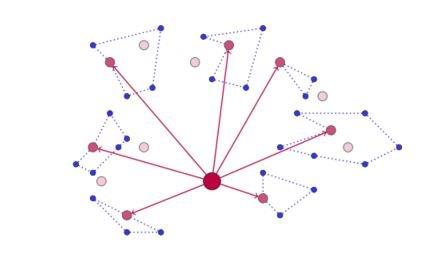
\includegraphics{Fig1.jpg}
\caption{\label{Exemple} \textbf{Exemple de solution possible de LIRP \cite{}}}
\end{figure}

\newpage



\subsection{Formulation mathématiques}
Cette formulation est issue du document de Olivier Peton \cite{} introduisant le Problème LIRP.
\subsubsection{Notations}\label{notations}
\begin{tabular}{ll}
\hline
Ensemble & Définition \\
\hline
$I$ & ensemble de clients\\ 
$J$ & ensemble de centres de distributions ou depôts\\
$P$ & ensemble d'usines (1 usine ici)\\
$T=\left \{0,...,|T|\right \}$ & ensemble de periodes (days)\\
$K$ & nombre de vehicule\\
$V$ & ensemble de sites $V=P\cup I \cup J$\\
$V^*$ & ensemble de depôts et de clients $V^*=I \cup J$\\
$R$ & ensemble de routes possible\\
\hline
\end{tabular}
\newpage
\begin{tabular}{ll}
\hline
Données & Definition \\
\hline
$f_j$ & Coût fixe d'ouverture du depôt $j\in J$\\ 
$Q$ & Capacité du Vehicule (homogènes, qui sont de même taille)\\ 
$d^t_i$ & Demande du client $i \in  I$ au temps $t \in \left \{1,...,|T| \right \}$\\
$h^t_i$ & Cout de stockage d'une unité du site $i \in V^*$ au temps $t\in T$\\
$I_{i0}$ & Inventaire initial $i \in V^*$\\
$c_j$ & Coût de livraison de depôt $j\in J$ \\
$c_r$ & Coût de livraison de la route $r\in R$\\
$\alpha_{ir}$ & 1 si la route $r \in R$ visite le site $i\in V^*$. 0 sinon\\
$I^{max}_i$ & Inventaire maximal du site $i\in V^*$ \\
\hline
\end{tabular}
\subsubsection{Variables}~\\
\begin{tabular}{ll}
\hline
\multicolumn{2}{l}{\textit{Variables Binares}}\\
$y_j$ & $\rightarrow$ 1 si le depôt $j$ is selectionné. 0 sinon \\
$z^t_r$ & $\rightarrow$ 1 si route $r \in R$ est selectionnée au temps $t\in T$. 0 sinon\\
$x^t_j$ & $\rightarrow$ 1 si le depôt $j\in J$ est selectionné au temps $t$. 0 sinon\\
\hline
\multicolumn{2}{l}{\textit{variables Continues}}\\
\hline
$q^t_j$ & $\rightarrow$ Quantité delivrée au depôt $j\in J$ au temps $t\in T$\\
$u^t_{ir}$ & $\rightarrow$ Quantité delivrée par la route $r\in R$ au client $i \in I$ dans le temps $t \in T$\\
$I^t_i$ & $\rightarrow$ Inventaire du site $i\in I\cup J$ au temps $t \in T$\\
\end{tabular}

\subsubsection{MIP defintion}
\begin{equation}
\text{min} \sum_{j\in J} f_j y_j 	+\sum_{t\in T} 
\left( \sum_{j\in J} c_j x^t_j + \sum_{r\in R} c_r z^t_r  + \sum_{t\in T} \sum_{i\in V^*} h^t_i I_i^t\right) \label{objfunct}\
\end{equation}

\begin{align}
\text{s.t.}  &&\sum_{r\in R} \alpha_{ir} z^t_r 	&\leq 1 					&\forall i\in I, \forall t\in T  \label{const:customersingleroute}\\
		&&q^t_j 								&\leq Q x^t_j				&\forall j\in J, \forall t\in T \label{const:plantcapacity}\\
		&&x^t_j 								&\leq y_j   				&\forall j\in J, \forall t\in T\label{const:nounselectedroutes}\\
		&&\sum_{i\in I} u^t_{ir}   				&\leq  Q z^t_r 				&\forall r\in R, t\in T\label{const:capacityonroute}\\
		&&\sum_{r\in R} z^t_r 					&\leq \begin{vmatrix} K \end{vmatrix} 					&\forall t\in T\label{const:fleetsizelimitation}\\
		&&z^t_r 								&\leq \sum_{j\in J}\alpha_{jr} y_j 				&\forall r\in R, \forall t\in T\label{const:routestartsfromDC}\\
		&&I^{t-1}_j + q^t_j   					&=I^t_j +\sum_{r\in R}\alpha_{jr} \left(\sum_{i\in I}u^t_{ir}\right) 	&\forall j\in J, \forall t\in T \label{const:flowconversationatDC}\\
		&&I^t_i				&=I^{t-1}_i+ \sum_{r\in R} u^t_{ir}-d^t_i 	&\forall i\in I, \forall t\in T\label{const:flowconservationatcustomer}\\
		&&I^t_i 			&\leq \min(I^{max}_i, \sum_{t'>t}^{t'<T}d^{t'}_i) 		&\forall i\in I, \forall t\in T\label{const:maxinventorycust}\\
		&&I^t_j									&\leq I^{max}_j y_j  				&\forall j\in J,\forall t\in T\label{const:capconstraintatdepot}\\	
		&&u_{ir}^t 			&\leq Q \alpha_{ir}						& \forall i\in I, \forall r\in R,\forall t\in T	\label{const:upperbound-u}\\
		&&q^t_j 						&\geq 0 					& \forall j\in J,\forall t\in T	\\
		&&u^t_{ir}						&\geq 0 					&\forall i\in I, \forall r\in R,\forall t\in T	\\
        &&y_{j}									& \in \{0,1\}, 				&\forall j\in J\label{12}\\	
		&&z^t_r									&\in \{0,1\}, 				&\forall r\in R, \forall t\in T						\label{13}\\
		&&x^t_{ij}								&\in \{0,1\},				&\forall i \in I, \forall j\in J,\forall t\in T		\label{14} \\
		&&I_i^t 								& \geq 0					&\forall i \in V^*, \forall t\in T \\
\end{align}

La fonction objective \eqref{objfunct} minimise le coût total : d'ouverture de sites, de la gestion de stocks et du coût de routage.
La contrainte \eqref{const:customersingleroute} fait état à ce que chaque client soit visité par au moins une route à un temps T. 
La contrainte \eqref{const:plantcapacity} est une contrainte de capacité sur la quantité de distribution de depôt qui depasse pas la quantité
maximale d'un vehicule.
La contrainte \eqref{const:nounselectedroutes} impose qu'un depôt est distribué si et seulement s'il est ouvert. 
La contrainte \eqref{const:capacityonroute} est une contrainte de capacité sur la quantité distribuée par une route qui ne depasse pas celle d'un vehicule.
La contrainte \eqref{const:fleetsizelimitation} impose une borne sur le nombre de route à utiliser à un instant T en fonction du nombre de vehicule.
La contrainte \eqref{const:routestartsfromDC} assure qu'une route passe par un et un seul depot ouvert si elle est selectionnée au temps T.
La contrainte \eqref{const:flowconversationatDC} est une conservation de flots d'inventaire au niveau des depôts.
La contrainte \eqref{const:flowconservationatcustomer} est une conservation de flots d'inventaire au niveau des clients. 
La contrainte \eqref{const:maxinventorycust} impose une borne superieure sur la quantité de stocks des clients au temps T.
La contrainte \eqref{const:capconstraintatdepot} impose une borne superieure sur la quantité de stocks des depôts au temps T.
La contrainte \eqref{const:upperbound-u} est une contrainte de capacité sur la quantité delivrée à un client connaissant la route et l'instant de livraison.





\section{Implémentation}
L'implémentation du model ci-dessus est réalisé en C à l'aide du solveur CPLEX. Les instances du problème étudiées lors des tests, sont composées de :
\begin{enumerate}
 \item Cinq clients, trois depôts en trois periodes
 \item Cinq clients, cinq depôts en cinq periodes
 \item Cinq clients, cinq depôts en sept periodes
 \item Sept clients, cinq depôts en cinq periodes
 \item Quinze clients, cinq depôts en cinq periodes
\end{enumerate}


\subsection{Les données d'instances}
Quant au donnée d'instances, on dispose des elements suivants en entrée :
\begin{itemize}
   \item Nombre de clients
   \item Nombre de depôts 
   \item Nombre de periodes 
   \item Nombre de vehicules
   \item Capacité du vehicule
   \item Coût par km
   \item Coût d'installation pour chaque depôt
   \item Coût de commande pour chaque depôt
   \item Quantité de stock initial pour chaque depôt et client
   \item Quantité de stock maximal pour chaque depôt et client
   \item Demande des clients en fonction du temps
   \item Coût de stockage d'une unité pour chaque depôt et client en fonction du temps,
	  on suppose que le couts de stockage change en fonction du temps
   \item Les coordonnées en deux dimensions des clients, depôts et de l'usine.
\end{itemize}

\paragraph{}
La dernière étape de la préparation des données est la generation des routes assurant la livraison. Pour s'y faire plusieurs méthodes nous est
offert comme la generation de toutes les combinaisons de routes possible, ce qui peut valoir des millions de routes lorsque la taille de l'instances
augmente. Par alleurs, on peut utiliser des heuristiques simples et limiter le nombre de routes à generer à un nombre de paramètre definit dans le 
fichier d'instances. Parmi ces paramètres, on peut citer :\\

\left\{
    \begin{tabular}{ll}
	CMAX & Nombre de clients maximal sur une route\\
	RMAX & Nombre de route maximale à generer\\
	LMAX & Coût maximal d'une route\\
	DMAX & Distance maximal entre un depôt de livraison et son client \\
    \end{tabular}
\right.

\paragraph{}
Lorqu'une route est generée, on teste si son coût est plus que LMAX et si c'est le cas, la route est abandonée. En outre quand la distance entre
un depôt et un client est superieure à DMAX alors il n'existera aucune route reliant ces deux sites.


\subsubsection*{Toutes les routes}
Cette option est interessante uniquement lorsque le paramètre CMAX sur une route n'est pas assez élevé pour pouvoir resoudre le modèle dans un temps raisonnable.
Le nombre de routes dans ce contexte vaut m * ($2^{CMAX} - 1$) dans le pire des cas où m est le nombre de depôts. On genere pour chaque
depôt, de 1 client à CMAX clients, une route.
    
    
\subsubsection*{heuristiques}
Dans le reste des cas, on genere RMAX routes possible en fonction de CMAX et DMAX. Quatres heuristiques sont élaborer :
\begin{itemize}
 \item Les routes choisis aleatoirement dans l'ensemble m * ($2^{CMAX} - 1$)
 \item Les routes les plus courtes de 1 client à CMAX clients en s'arretant lorsque RMAX est atteint
 \item Les routes les plus longues de CMAX clients à 1 client en s'arretant lorsque RMAX est atteint
 \item Les routes par paquet : ici, on prend toutes les routes , m * ($2^{CMAX} - 1$) en les fractionnant par paquet de taille RMAX. Les paquets sont 
 construits aleatoirement. On lance le modèle  sur chaque paquet de route et l'union des routes selectionnées pour chaque paquet forme `` les routes 
 generées '' sur lesquelles le model est relancé pour avoir de bonnes solutions sinon la solution optimale.
 On constate que le dernier paquet peut avoir une taille plus petite que RMAX et peut arriver à provoquer la non faisabilité du modèle 
 sur ce dernier.
 
\end{itemize}

\textbf{Remarque} : m * ($2^{CMAX} - 1$) est la taille de toutes les routes possible en fonction de l'instances d'entrée dans le pire des cas possible vu que grâce
à DMAX, on élague certains routes de l'ensemble. La valeur de CMAX est toujours plus petit ou egale à n.

\subsection{Exécution}

\section{Conclusion}

Conclusion

\section{Annexe}

Annexe

\section*{R\'emerciements}
\newpage
\bibliographystyle{unsrt}
\bibliography{rapport}
\end{document}